\section{Results}
\numberwithin{equation}{section}


\subsection{Benchmark of values}

\begin{itemize}

  \item \textbf{Image: gain VS time for one single point. Overlay between
    experiment/daniels sim/our sim}

  \item comparison with previous values from Daniel's thesis

  \item (comparison with results from an experiment)

\end{itemize}



\subsection{Runtimes}
In Figure \ref{plot:runtime}, the developed parallel ASE-flux algorithm was compared to 
the original single threaded algorithm in
\cite{ASE2010}. The mesh was sampled with an increasing number of rays per sample
to show linear scaling of the algorithm. Using four GPUs, a speedup of up to 
296 (84 for one GPU) was reached. However, the GPU algorithm was enhanced with
more features during development process, resulting in more complex computations.
\begin{figure}[H]
  \centerline{
    \resizebox{0.5\textwidth}{!}{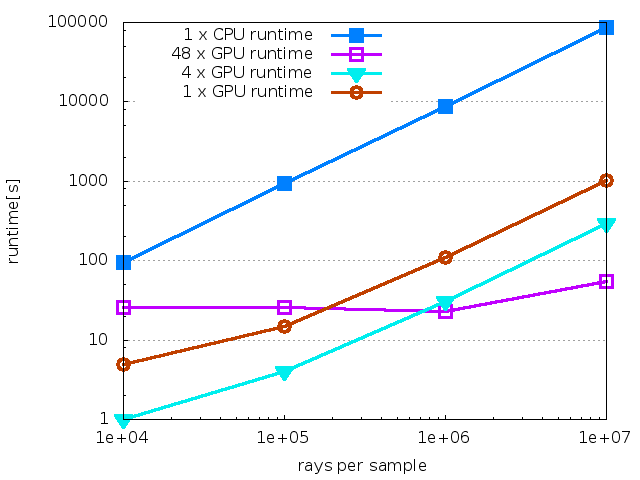
\includegraphics{plot/runtime.png}}}
  \caption{runtime of orginial algorithm compared to parallel algorithm}
  \label{plot:runtime}
\end{figure}
Distributing the computation to multiple devices scales well up to the
point, that every sample point is simulated with the exact same number
of rays. Changing this (e.g. through adaptive sampling), leads to
a potencial unbalanced distribution of computation and therefore to
a worse scaling (Figure \ref{plot:gpu_scaling}).
\begin{figure}[H]
  \centerline{
    \resizebox{0.5\textwidth}{!}{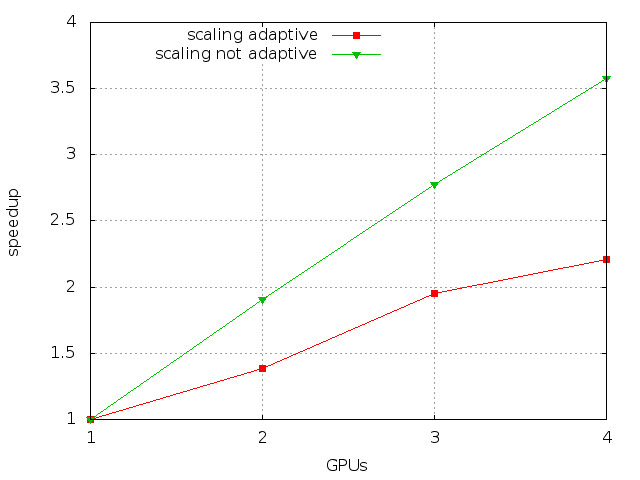
\includegraphics{plot/scaling.png}}}
  \caption{scaling on multiple devices}
  \label{plot:gpu_scaling}
\end{figure}
But nevertheless, by introducing adaptive sampling, the precision of the the simulation
can be adjusted by a $MSE$-threshold rather than increasing the number
of rays for every sample point. By making the attempt to stay under this $MSE$-threshold,
the maximal $MSE$ values decreases very fast. Thus very low computation time results in
simulation values comperable to extremly long simulations (see Figure \ref{plot:adaptive_runtime}).
\begin{figure}[H]
  \centerline{
    \resizebox{0.5\textwidth}{!}{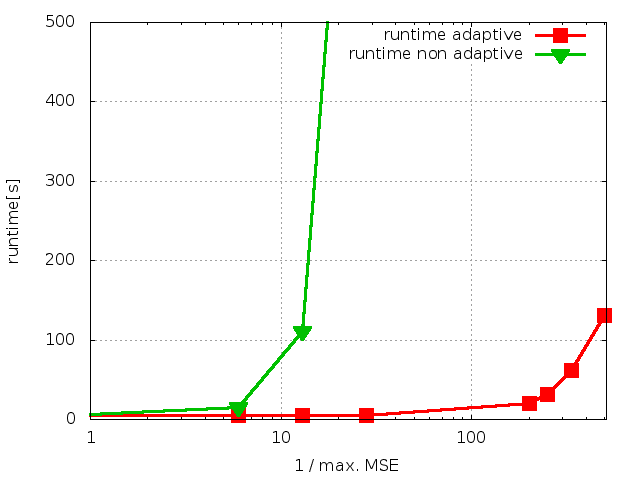
\includegraphics{plot/adaptive_runtime.png}}}
  \caption{runtime comparison of adaptive and non adaptive }
  \label{plot:adaptive_runtime}
\end{figure}

\subsection{Limitations and future work}
\label{subsec:limitations}
Future work should address reflections on the sides of the gain medium to allow the
simulation of lateral lasing. The current implementation only supports
reflections on the upper and lower surface.
Apart from that, the scaling issues seen in Figure \ref{plot:gpu_scaling} can be
mitigated by assigning the samplepoints to the GPUs in a demand-based way.  In
theory, processing times on the different devices will be more evenly, reducing
the time needed to wait for the slowest device and thus decreasing the
cumulative duration of the calculation. Having such a system in place, one might
easily extend the algorithm to span over multiple nodes in a cluster using
Message Passing Interface (MPI)\cite{MPI} to further increase the speed.
